\documentclass[]{scrartcl}

\usepackage{amsmath,amssymb}
\usepackage{graphicx}
\usepackage{tikz}

%opening
\title{Optimal design of experiment}
\author{Oliwer Sliczniuk}

\begin{document}

\maketitle

\begin{abstract}
Notes about the optimal design of an experiment
\end{abstract}

\section{What information do we have?}

\begin{itemize}
	\item Process model: $\dot{x}=f(t,x,p)$
	\item Measurement equation: $\dot{y}=g(x)$
	\item Likelihood function with respect to the dataset
	\item Parameter estimation
	\item Sensitivity equations: $\dot{S} = J_x \dot{x} + J_p$
\end{itemize}

\section{Maximum likelihood}
Let $y^s$ be the vector of all experimental results (random vector) to be used to estimate parameters $p$ and model output $y^m(p)$. The vector of the corresponding quantities computed by the model $\dot{x}=f(t,x,p)$. For a parallel model, the parameters of which are to be estimated from measurements of an output vector $\dot{y}=g(x)$. We shall call any optimizer of $j$, i.e., any $\hat{p}$ that corresponds to an optimal value of the cost function $j$, an estimate of $p$ in the sense of $j$.

The vector $\hat{p}_{ml}$ will be a maximum-likelihood estimate if it maximizes the cost function:

\begin{equation}
	j_{ml} = \pi_y (y^s|p) 
\end{equation}

If $p$ were fixed, $\pi_y(y^s|p)$ would be the probability density of the random vector $y^s$ generated by a model with parameters $p$. Here, to the contrary, $y^s$ is fixed and corresponds to the observations. Considered as a function of $p$, $\pi_y(y^s|p)$ is then called the likelihood of $y^s$. The maximum-likelihood method looks for the parameter vector $p$ value that gives the observed data the highest likelihood. In practice, it is often easier to look for $\hat{p}_{ml}$ by maximizing the log-likelihood function, yielding the same estimate since the logarithm function is monotonically increasing.

\begin{equation}
	j_{ml} = \ln ( \pi_y (y^s|p) )
\end{equation}

Assume that the observed outputs satisfy 

\begin{equation}
	y(t_i) = y^m(t_i, p^*) + \epsilon_i, \qquad i=1,...,n_t
\end{equation}

where the vector $y^m(t_i. p^*)$ is the output of a deterministic model, $p^*$ is the true value of the parameter vector, and $\epsilon_i$ belongs to a sequence of independent random variables with probability density $\pi_{\epsilon}(\epsilon_i)$. Since the $\epsilon_i$ are independent

\begin{equation}
	\pi_{\epsilon}(\epsilon_1, \epsilon_2, ..., \epsilon_{n_t}) = \prod_{i=1}^{n_t} \pi_{\epsilon_i}(\epsilon_i)
\end{equation}

Consider the output error

\begin{equation}
	e^y(t_i, p) = y(t_i) - y^m(t_i, p)
\end{equation}

For the true value of the parameters, it satisfies $e^y(t_i, p^*)=\epsilon_i$. and, since $y^m$ is deterministic, $\pi_{y_i} (y^s(t_i)|p) = \pi_{\epsilon_i} (e^y(t_i)|p)$. The likelihood of the $n_t$ observations can be written as

\begin{equation}
	\pi_y (y^s|p) = \prod_{i=1}^{n_t} \pi_{\epsilon_i}(e^y(t_i,p)) =  \prod_{i=1}^{n_t} \pi_{\epsilon_i}(y(t_i) - y^m(t_i, p))
\end{equation}

If the noise is assumed to follow the normal distribution with the standard deviation $\sigma$, which is known from the parameter estimation:

\begin{equation}
	\pi_y (y^s|p) = \prod_{i=1}^{n_t} \frac{1}{ \sqrt{2\pi\sigma_{t_i}^2} } \exp \left( -\frac{1}{2} \left( \frac{y(t_i) - y^m(t_i, p)}{\sigma_{t_i}} \right)^2 \right)
\end{equation}

The associated log-likelihood can be written as

\begin{equation}
	\ln (\pi_y (y^s|p)) = (\text{term independent of p}) - \frac{1}{2} \sum_{i=1}^{n_t}  \left( \frac{y(t_i) - y^m(t_i, p)}{\sigma_{t_i}} \right)^2
\end{equation}

Its gradient is thus

\begin{equation}
	\frac{\partial}{\partial p} \ln (\pi_y (y^s|p)) =  \sum_{i=1}^{n_t}  \left[ \left( \frac{y(t_i) - y^m(t_i, p)}{\sigma_{t_i}^2} \right) \frac{\partial y^m(t_i, p)}{\partial p} \right]
\end{equation}

\section{Fisher information}

The Fisher information is a way of measuring the amount of information that an observable random variable carries about an unknown parameter of a distribution that models the random variable. The Fisher information is related to the second derivative (or the curvature) of the log-likelihood function with respect to the parameter. This relationship provides a measure of how "sensitive" the likelihood is to changes in the parameter value. The Fisher information matrix can be calculated as follow.

\begin{align}
	F(p) &= - \mathop{\mathbb{E}}_{y^s|p} \left[ \frac{\partial^2 \ln (\pi_y (y^s|p))}{\partial p \partial p^T} \right] = \mathop{\mathbb{E}}_{y^s|p} \left[ \frac{\partial \ln (\pi_y (y^s|p))}{\partial p} \frac{\partial \ln (\pi_y (y^s|p))}{\partial p^T} \right] \\
	&= \mathop{\mathbb{E}}_{y^s|p} \left[ \sum_{k=1}^{n_t} \left( \frac{y(t_k) - y^m(t_k, p)}{\sigma_{t_k}^2} \frac{\partial y^m(t_k, p)}{\partial p} \right) \times  \sum_{i=1}^{n_t} \left( \frac{y(t_i) - y^m(t_i, p)}{\sigma_{t_i}^2} \frac{\partial y^m(t_i, p)}{\partial p^T} \right) \right]
\end{align}

Considering the mismatch between the dataset and the model output, the expectation becomes $\mathop{\mathbb{E}}_{y^s|p} \left[ \left( y(t_i) - y^m(t_k, p) \right) \right] = \mathop{\mathbb{E}}_{y^s|p} \left[ \epsilon_i^2 \right]$. For $i=k$, the expectation of $\epsilon_i$ is the variance of the noise $\sigma_{t_i}^2$. Analogously, the expectation becomes 0 if $i \neq k$ because the expectation of the noise $\epsilon_i$ is zero and the measurements are independent at different times.

\begin{equation}
	\mathop{\mathbb{E}}_{y^s|p} \left[ \left( y(t_i) - y^m(t_k, p) \right) \left( y(t_i) - y^m(t_i, p) \right) \right] = \sigma_{t_i}^2 \delta_{ik}
\end{equation}

where $\delta_{ik}$ represents the Kronecker delta. Given the property of the Kronecker delta, the double summation in the Fisher Information matrix reduces to a single summation:

\begin{equation}
	F(p) = \sum_{i=1}^{n_t} \left( \frac{1}{\sigma_{t_i}^2} \frac{\partial y^m(t_i, p)}{\partial p} \frac{\partial y^m(t_i, p)}{\partial p^T} \right)
\end{equation}

If every experiment at time $t_i$ is independent and characterized by its own $\sigma_{t_i}$, then the Fisher information matrix can be presented in the more compact way:

\begin{equation}
	F(p) = \frac{\partial y^m(t, p)}{\partial p} \begin{bmatrix}
		\frac{1}{\sigma_{t_1}^2} & 0 & 0\\
		0 & \ddots & 0 \\
		0 & 0 & \frac{1}{\sigma_{t_{n_t}}^2} 
	\end{bmatrix}\ \frac{\partial y^m(t, p)}{\partial p^T} 
\end{equation}

\section{Cramer-Rao inequality}

Let $\hat{p}$ be an (absolutely) unbiased estimator $p^*$, i.e. such that it were possible to replicate the same experiment and estimate $\hat{p}$ an infinite number of times, the mean of the estimates would coincide with the true value. Let $P$ be the covariance matrix of this estimator. Since $\hat{p}$ is unbiased, $P$ can be written as

\begin{equation}
	P = \mathop{\mathbb{E}}_{y^s|p^*} \left[ \left( \hat{p}(y^s) - p^* \right) \left( \hat{p}(y^s) - p^* \right)^T \right]
\end{equation}

which quantifies how the estimates are spread around the true value $p^*$. One would like the estimates to be as concentrated as possible around this true value. An estimator $\hat{p}_1$ with covariance matrix $P_1$ is said to be more efficient than an estimator $\hat{p}_2$ with covariance matrix $P_2$ if $P_1 < P_2$, that is if $P_2 - P_1$ is positive-definite (i.e.if all the eigenvalues of $P_2-P_1$ arc strictly positive). Since estimators with high efficiency are desirable, a natural request is to make P as small as possible. The Cramer-Rao inequality provides a lower bound to what can be achieved.

Under the hypotheses that:

\begin{itemize}
	\item the set of all data vectors $y^s$ with $\pi_y(y^s|p) > 0$ does not depend on $p$
	\item $\frac{\partial \pi_y(y^s|p)}{\partial p_i}~\left(i=1,2,...,n_p\right)$ is absolutely integrable
	\item $\mathop{\mathbb{E}}_{y^s|p} \left[ \frac{\partial \ln (\pi_y (y^s|p))}{\partial p} \frac{\partial \ln (\pi_y (y^s|p))}{\partial p^T} \right]$ exists and is invertible
\end{itemize}

the covariance of any absolutely unbiased estimator satisfies

\begin{equation}
	P \geq F^{-1}(p^*)
\end{equation}

In other words, the precision to which we can estimate $p$ is fundamentally limited by the Fisher information of the likelihood function. Based on the Cramer-Rao inequality, the Fisher information matrix can used to calculate the covariance matrices associated with maximum-likelihood estimates.

\section{Optimal experimental design}

The optimal design of experiments (DOE) is a statistical concept that refers to the process of planning an experiment, which allow parameters to be estimated without bias and with minimum variance. Optimal design ensures that the experiment can provide the most informative data possible. This often involves balancing the study of main effects and interactions between factors. Moreover, by efficiently planning experiments, optimal design aims to reduce the overall resources required, such as time, materials, and manpower.

The methodology for data to estimate the parameters of a specific model is influenced by a series of qualitative decisions made throughout the experimental and modelling process, such as: a model structure, a location of sensors or an equipment. Once these choices have been made, the experimenter still has some freedom to specify the quantitative experimental conditions (such as temperature, pressure, sampling times, etc.). Experiment design aims to determine experimental conditions adapted to the final purpose of the modeling. 

%Assume that the i'th scalar observation can be written as $y(\xi_i)$, where the $n_\xi$-dimensional vector $\xi_i$ (the i'th support point) describes the experimental conditions (e.g., measurement time, the shape of input, etc.) under which the i'th observation is to be collected. When $n_t$ such observations are taken, the concatenation of the vectors $\xi_i$'s yields the $\Xi = (\xi_1, \xi_2,..., \xi_{n_t})$, which characterizes all experimental conditions to be optimized. To make the experiment design realistic, it is necessary to consider several constraints, e.g., the experiments' duration, the inlet stream's temperature, and the minimum time between samples. Let $\bar{\Xi}$ be the set of all feasible values for $\Xi$. 

Let's consider that each scalar observation in our study can be expressed as $y(\xi_i)$, where the $n_\xi$-dimensional vector $\xi_i$ representing the specific experimental conditions (such as the timing of measurements, operating conditions, etc.) under which the i'th observation is gathered. When collecting $n_t$ such observations, the assembly of these $\xi_i$ vectors forms the matrix $\Xi = (\xi_1, \xi_2,..., \xi_{n_t})$, which combine all the experimental conditions that need optimization. In order to align the design of the experiment with practical realities, it's important to take into account various constraints, such as the total duration of the experiments, the maximum temperature of the inlet stream, and the minimum interval between sampling events. The set of all possible combinations for $\bar{\Xi}$ that adhere to these constraints is denoted as $\Xi$.

%The definition of a cost function $j$ then permits the optimal experiment design to be cast as a constrained optimization problem, where the optimal experiment $\Xi^*$ is defined by

The formulation of a cost function $j$ allows for the framing of optimal experiment design as a problem of constrained optimization. In this context, the optimal experiment, denoted as $\Xi^*$:

\begin{equation}
	\Xi^* = \arg~\underset{\Xi \in \bar{\Xi}}{\text{opt}}~j\left(\Xi\right)
\end{equation}

The cost function should describe the amount of information from an experiment. For that purpose it can be assumed a function $\phi$ can be related to the Fisher information obtained an arbitrary operating conditions.

\begin{equation}
	j(\Xi) = \phi\left[ F(p, \Xi) \right]
\end{equation}

%Under the hypotheses mentioned above, the distribution of the maximum likelihood estimator is asymptotically Gaussian $\mathop{\mathbb{N}} (p^*, F^{-1}([^*, \Xi])) $ when the number of measurements tends to infinity. Minimizing $j(\Xi)$ then amounts to minimizing a scalar measure of the asymptotic covariance matrix of the parameters.

A general class of optimality criteria for DOE is given by

\begin{align}
	\phi_k(F) &= \left[\frac{1}{n_p} \text{trace}\left( QF^{-1}Q^T \right)^k \right]^{1/k} \quad &if \det F \neq 0 \nonumber \\
	\phi_k(F) &= \infty \quad &if \det F = 0
\end{align}

where $Q$ is a weighting matrix. The special case $k = 1$ corresponds to the L-optimality cost function,

\begin{equation}
	j_L(\Xi) = \text{trace} \left[ Q^TQF^{-1}(p,\Xi) \right]
\end{equation}

and choosing $Q = \textbf{I}_{n_p}$ then corresponds to the A-optimality cost function. An A-optimal experiment minimizes the sum of the squares of the lengths or the axes of asymptotic confidence ellipsoids. Choosing $Q$ diagonal, with $[Q]_{ii} = 1/p_i$ corresponds to C-optimality, which is connected with the relative precision of estimates. Taking Q to be a row vector leads to c-optimality. Taking $Q = \textbf{I}_{n_p}$ and $k = \infty$ corresponds to E-optimality; E-optimal design maximizes the smallest eigenvalues of the Fisher information matrix and thus minimizes the length of the largest axis of the asymptotic confidence ellipsoids. The most widely used optimality criterion has $k = 0$, $Q = \textbf{I}_{n_p}$ , requiring minimization of $\det F^{-1}(p, \Xi)$, or, equivalently, maximization of

\begin{equation}
	j_D(\Xi) = \det F(p, \Xi)
\end{equation}

A D-optimal experiment minimizes the volume of the asymptotic confidence ellipsoids for the parameters. The graphical representation of the different optimality conditions is shown in Figure \ref{fig:score_fun}.

\begin{figure}[!h]
	\centering
	\resizebox{0.4\textwidth}{!}{%
	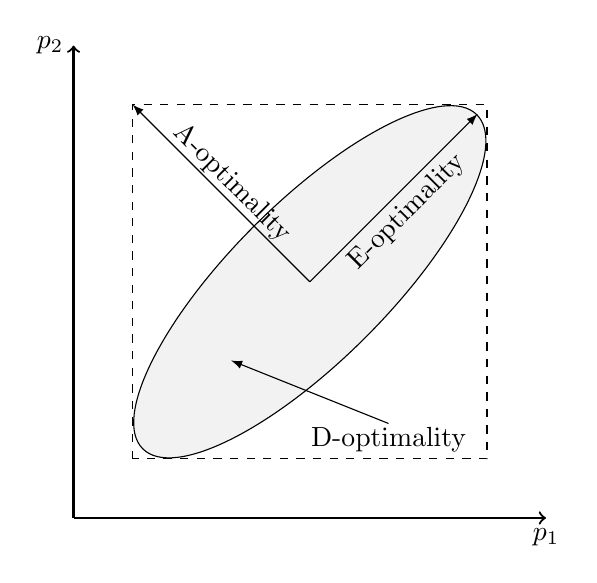
\begin{tikzpicture}
		% Ellipse parameters
		\def\ellipsecenter{(3,3)}
		\def\ellipseA{(0.75,5.25)} % End point for A-optimality arrow
		\def\ellipseB{(5.13,5.13)} % End point for E-optimality arrow
		\def\ellipseC{(4,1.2)}      % End point for D-optimality arrow
		
		% Draw the rotated ellipse
		\draw[fill=gray!10, draw=black, rotate around={45:\ellipsecenter}] \ellipsecenter ellipse (3cm and 1cm);
		
		% Draw the dashed rectangle
		\draw[dashed] (0.75,0.75) rectangle (5.25,5.25);
		
		% Draw the arrows and label them with adjustable positions
		\draw [-latex] \ellipsecenter -- \ellipseA node[yshift=-4cm, xshift=2.5cm,rotate around={-45:\ellipsecenter}] {A-optimality};
		\draw [-latex] \ellipsecenter -- \ellipseB node[yshift=0cm, xshift=-3.9cm,rotate around={45:\ellipsecenter}] {E-optimality};
		\draw [-latex] \ellipseC -- (2,2) node[yshift=-1cm, xshift=2cm] {D-optimality};
		
		% Draw axes
		\draw[thick,->] (0,0) -- (6,0) node[below] {$p_1$};
		\draw[thick,->] (0,0) -- (0,6) node[left] {$p_2$};
	\end{tikzpicture}
	}%
	\caption{Graphical representation of score functions}
	\label{fig:score_fun}
\end{figure}

\section{Problem formulation}

The optimal design of experiment technique is used extend the experiment discussed in ${\color{red}article~1}$, where supercritical extraction from caraway seeds has been discussed. In this work, the extraction has been performed at multiple operating conditions, such that the temperature, pressure and flow-rate were constant during each batch. Later, the results from all the experiments are combined and correlations for extraction kinetic parameters are presented. In this work, the optimal design of experiment is used to design an experiment to validate these correlations. The model parameters and the sampling time are the same as in ${\color{red}article~1}$ to mimic the original system. It is assumed that the flow-rate is constant, because the effect of the flow-rate has not been deeply investigated. The inlet temperature can be controlled by a controller 

\begin{equation}
	\begin{aligned} 
		&\hat{{\color{black} \theta}}_{MLE} &= \arg \max_{{\color{black} \sigma}, {\color{black} \theta} \in \Theta} \ln L = \arg \max_{{\color{black} \sigma},{\color{black} \theta} \in \Theta} p({\color{black} \theta}|{\color{black}y}) \\
		&\text{subject to}
		& \dot{ {\color{black}x} } = {\color{black}G}({\color{black} x}(t);{\color{black} \theta}) \\
		&& {\color{black} \dot{\theta}} = 0 \\
		&& {\color{black}y} = {\color{black}y}(t) \\
		&& {\color{black} \theta}^{lb} \leq {\color{black} \theta} \leq {\color{black} \theta}^{ub}
	\end{aligned}
\end{equation} 

\end{document}

































